\documentclass[tikz,border=10pt]{standalone}
\begin{document}
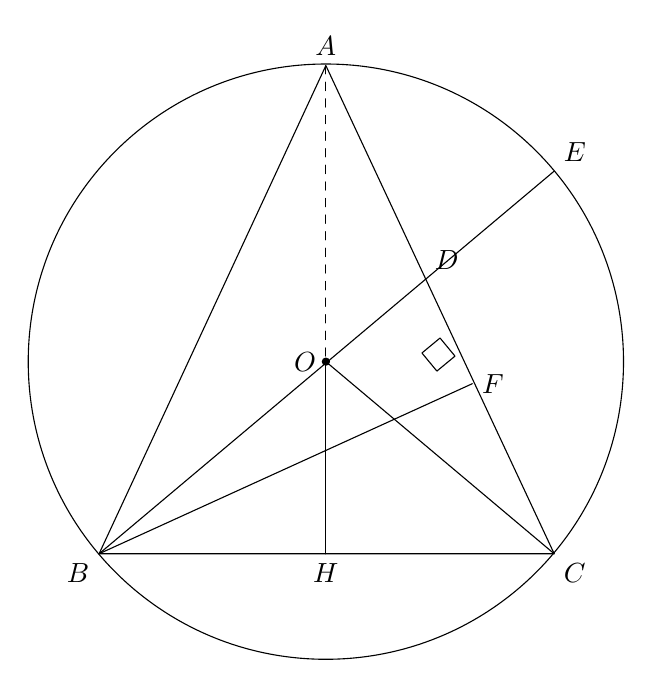
\begin{tikzpicture}[scale=1, line cap=round, line join=round]

% Points
\coordinate (A) at (2.88,6.2);
\coordinate (B) at (0,0);
\coordinate (C) at (5.78,0);
\coordinate (H) at (2.88,0);
\coordinate (O) at (2.88,2.44);
\coordinate (D) at (4.14,3.48);
\coordinate (E) at (5.78,4.86);
\coordinate (F) at (4.74,2.16);

% Circumcircle
\draw (O) circle (3.78);

% Triangle
\draw (A) -- (B) -- (C) -- cycle;

% Altitude AH (dashed above O, solid below O)
\draw[dashed] (A) -- (O);
\draw (O) -- (H);

% Line through B, O, D, E
\draw (B) -- (E);

% Other segments
\draw (O) -- (C);
\draw (B) -- (F);

% Right angle mark
\draw (4.1,2.55) -- (4.33,2.74) -- (4.52,2.51) -- (4.29,2.32) -- cycle;

% Labels
\node[above] at (A) {$A$};
\node[below left] at (B) {$B$};
\node[below right] at (C) {$C$};
\node[below] at (H) {$H$};
\node[left] at (O) {$O$};
\node[above right] at (D) {$D$};
\node[above right] at (E) {$E$};
\node[right] at (F) {$F$};

\fill (O) circle (1.5pt);

\end{tikzpicture}
\end{document}
